\begin{figure*}[H]
    \centering

    \subfloat[\Sh]{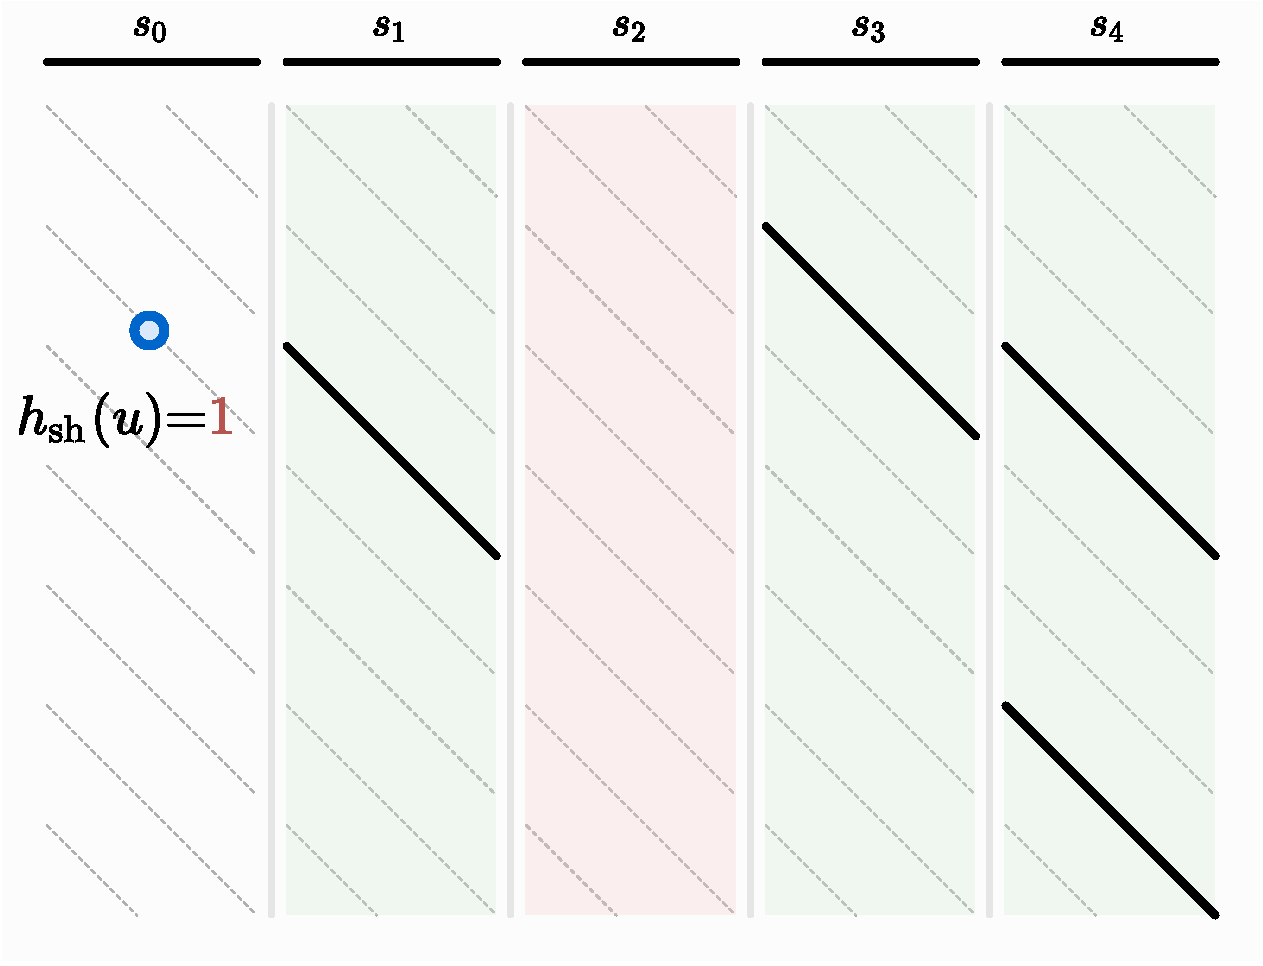
\includegraphics[width=0.31\linewidth]{imgs/fig2/sh.pdf}\label{GLOBALfig:sh}}
    \hfill
    \subfloat[\Csh]{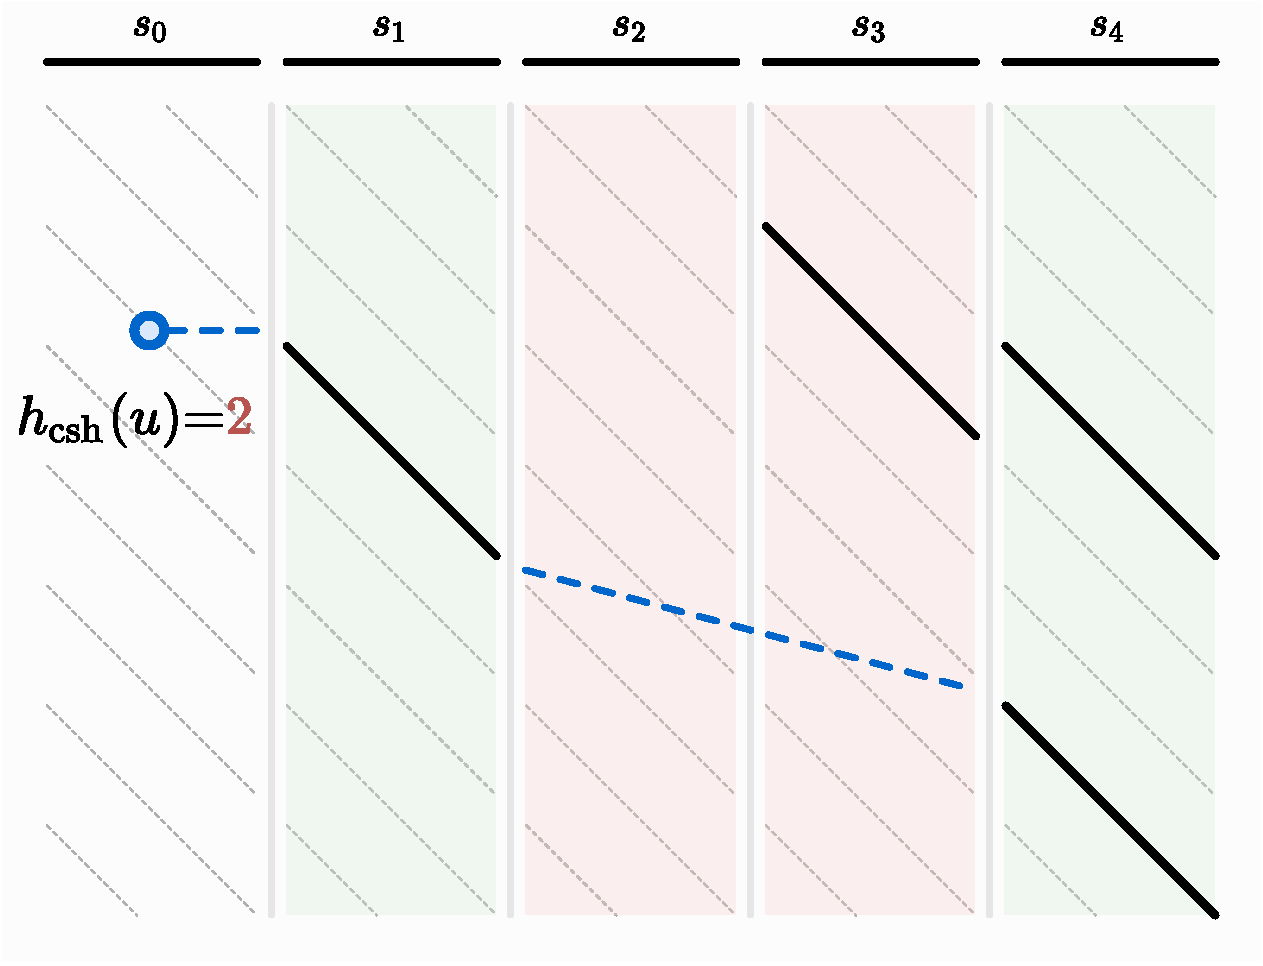
\includegraphics[width=0.31\linewidth]{imgs/fig2/csh.pdf}\label{GLOBALfig:csh}}
    \hfill
    \subfloat[\Csh + match pruning]{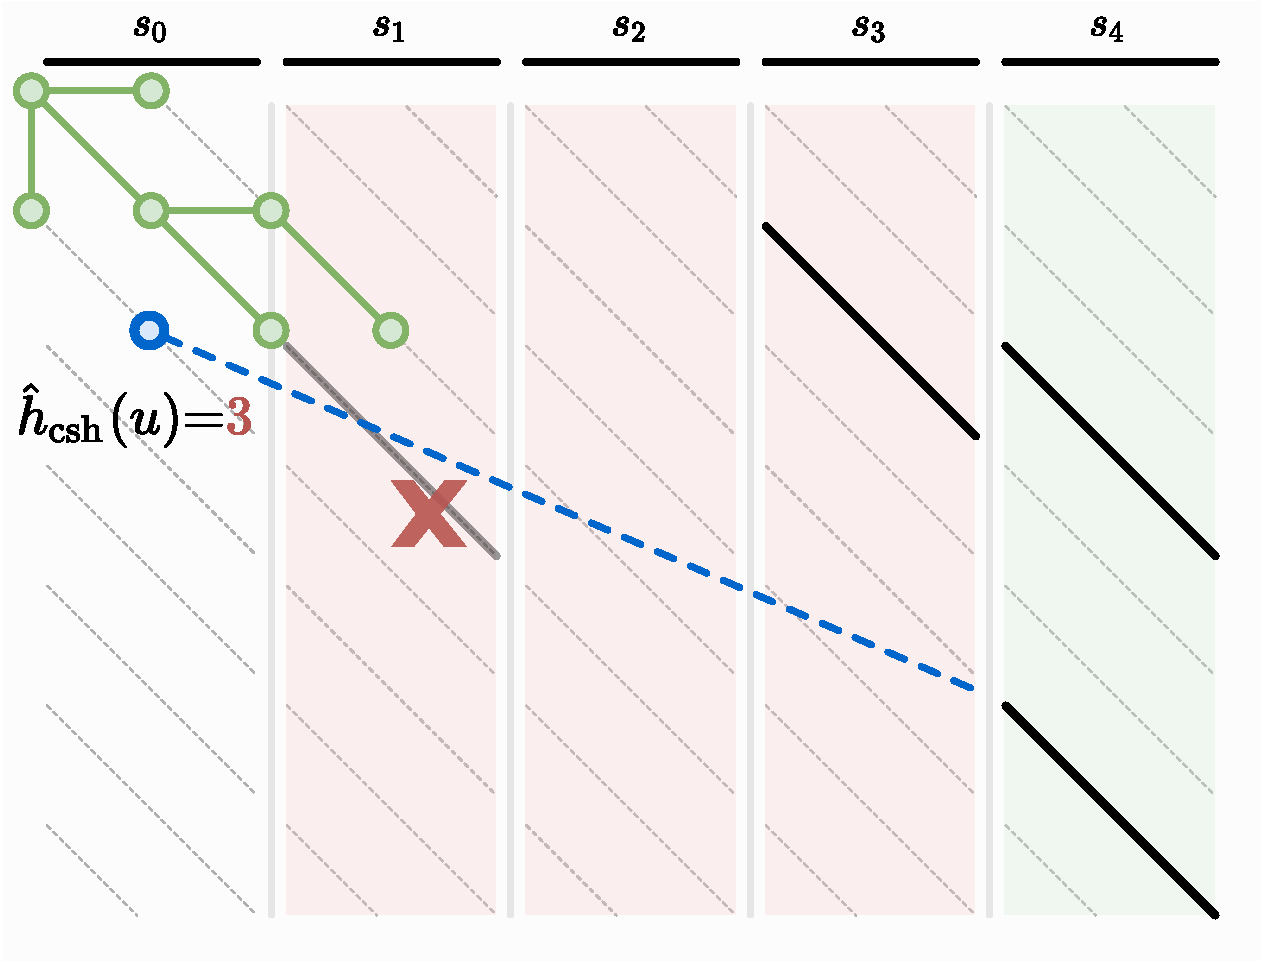
\includegraphics[width=0.31\linewidth]{imgs/fig2/pruning.pdf}\label{GLOBALfig:pruning}}

    \caption[Seed heuristic, match chaining, match pruning]{A demonstration of the \sh, \csh, and match pruning. Sequence $A$
      is split into $5$ seeds drawn as horizontal black segments (\seed) on top.
      Their exact matches in $B$ are drawn as diagonal black segments (\match). The
      heuristic is evaluated at the blue state ($u$, \bluecircle), based on the $4$ remaining
      seeds. The dashed blue paths show maximal length chains of seed matches
      (green columns, \greencolumn). The seeds that are not matched (red
      columns, \redcolumn) count
      towards the heuristic.
      %
      \protect\subref{GLOBALfig:sh} The \sh $\hsh(u) = 1$ is the number of remaining
      seeds that do not have matches ($s_2$).
      %
      \protect\subref{GLOBALfig:csh} The \csh $\hcsh(u) = 2$ is the number of not
      matched remaining seeds ($s_2$ and $s_3$) for a path going only down and
      to the right containing a maximal number of matches.
      %
      \protect\subref{GLOBALfig:pruning} Once the start of a match is expanded (shown
      as green circles, \greencircle), the match is \emph{pruned} (marked with
      red cross, \cross), and future computations of the heuristic ignore it.
      This reduces the maximum chain of matches starting at $u$ by $1$ ($s_1$)
      so that $\hcshS(u)$ increases by $1$. }
    \label{GLOBALfig:heuristics}
\end{figure*}
